%!TEX root = ../thesis.tex
%*******************************************************************************
%****************************** Second Chapter *********************************
%*******************************************************************************
\chapter{Associative STL containers} 
\graphicspath{{./Chapter2/Figs/}}

\section{Introduction} % section 2.1
\texttt{Associative containers} are containers in which every element stored inside is accessible 
by a special value called a \textbf{key}.

Therefore, there is an association between the element and the key. In \texttt{sequence containers}, elements 
are accessed by their place (index) in the container.

Associative containers are usually implemented on the basis of \textbf{binary search tree algorithms}, 
or even balanced binary trees. This makes them efficient storage containers, but usually quite big ones 
in comparison to other collections. In some rare cases this might be an issue.

There are \textbf{four} types of \texttt{associative containers} in the STL:
\begin{itemize}
  \item \texttt{set}
  \item \texttt{multiset}
  \item \texttt{map}
  \item \texttt{multimap}
\end{itemize}
In fact, there is the \textbf{bitset} too, but we’ll skip it in this tutorial. As you’ll see in the table on 
the following slide, all associative containers have a very similar interface, yet there are some 
fundamental differences between the \texttt{set} and \texttt{map} concepts.

The table shows the most important operations provided by STL associative containers. 
As you can see, the majority of the methods are common between the different types of containers.

\begin{figure}[htbp!]
  \centering
  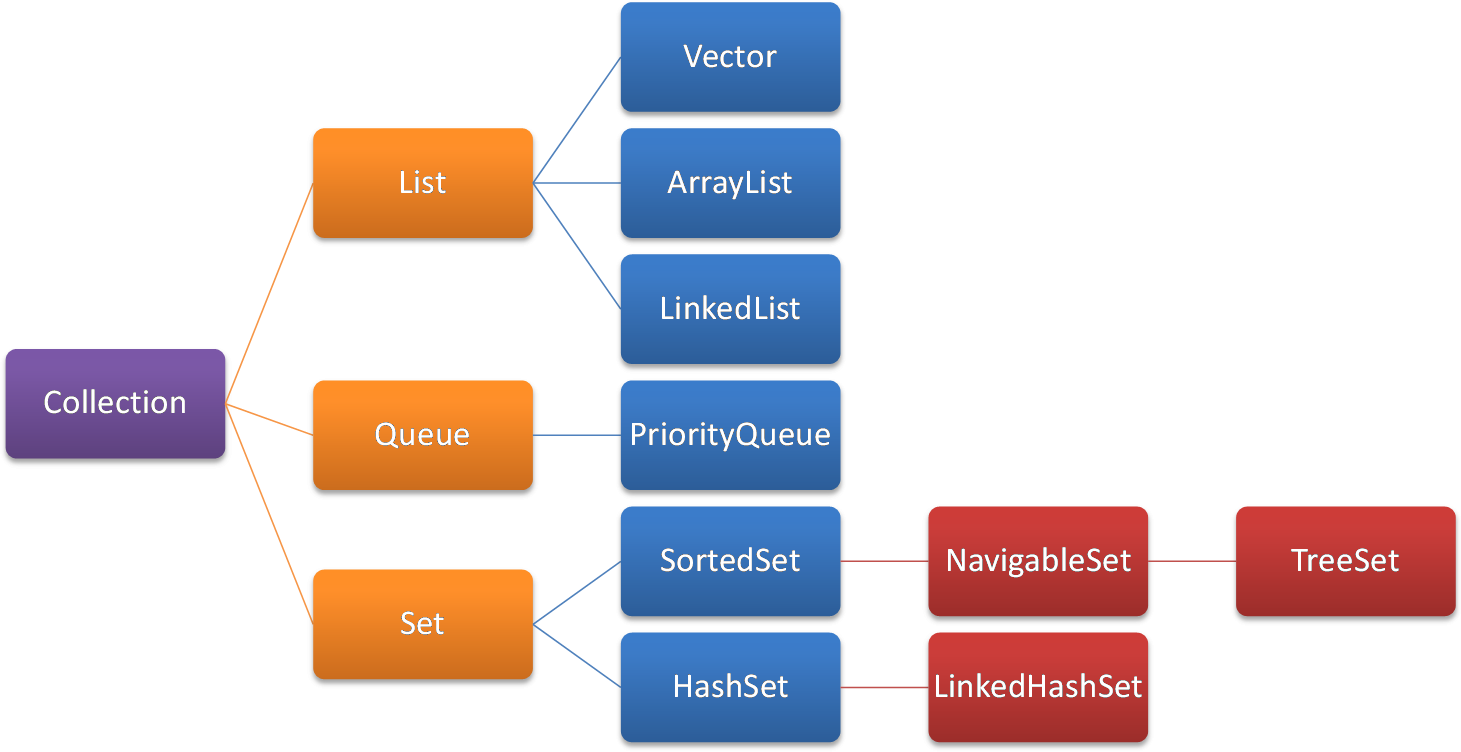
\includegraphics[width=1.0\textwidth]{set221}
  \caption[function]{Function table}
  \label{fig:function set}
\end{figure}

\section{Set and multiset} %section 2.2
\subsection{Template definition} %subsection 2.2.1
Below you can see the template definition of the \texttt{set} and \texttt{multiset} classes. 
Both classes are located in the same header file.
\begin{methodinfo}
  {<set>}
  {template < class Key, class Compare = less<Key>, class Allocator = allocator<Key> > class set;
  template < class Key, class Compare = less<Key>, class Allocator = allocator<Key> > class multiset;}
  {\texttt{Key} – the type of key stored inside the set, and therefore the type of the elements themselves

  \texttt{Compare} – the type of comparator used to perform a comparison between the \texttt{set} elements, 
  in order to ensure strict weak ordering. It can be implemented as a two-argument function, 
  or a functional object. If no comparator is provided, \texttt{less()} will be used as a default;

  \texttt{Allocator} – the type of allocator used to provide the storage allocation model.}
  {None}
  {\texttt{Set} and \texttt{multiset} are associative containers in which the elements stored 
  inside them are \texttt{keys} themselves.}
\end{methodinfo}

\subsection{Set and multiset functionality} %subsection 2.2.2
All \texttt{set} features are grouped in the table on the slide.

As you can see, there’s only one difference between these two classes, and this is why they’ll be 
described together. We’ll simply refer to both containers as \texttt{set} in the rest of this tutorial, 
with some exceptions, when their functionality differs.
\begin{figure}[htbp!]
  \centering
  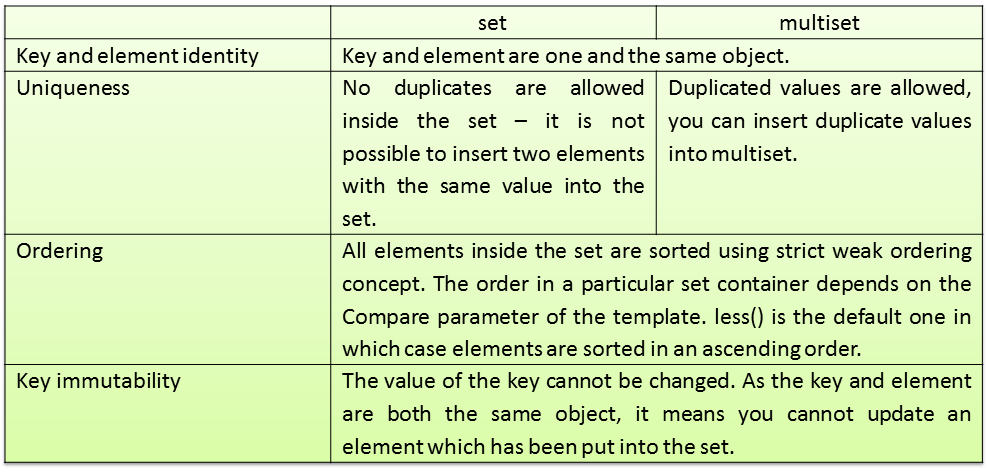
\includegraphics[width=1.0\textwidth]{set222}
  \caption[function]{Function table}
  \label{fig:function set}
\end{figure}

\subsection{Strict weak ordering \& the comparator object} %subsection 2.2.3
The elements inside the \texttt{set} are sorted using a strict weak ordering algorithm. 
In order for that to happen, two consecutive elements must be compared to one another. 
The comparison is performed using the second template parameter – \texttt{Compare}.

As you can see, the default value of that argument is \texttt{less<Key>}. In order for it to work, 
\texttt{less<Key>} requires the operator < to be defined for the type \texttt{Key}. If a particular type 
does not support this operation, a custom comparator must be created and passed during the \texttt{set} 
object definition.

Another reason to create a custom comparator is to provide some specific ordering.

A comparator \texttt{object} is required for the \texttt{set} and \texttt{multiset} to properly order the elements.

On the slide, you can see two possible prototypes of a comparator. The comparator should return \texttt{true} 
if the element k1 is placed before the element k2. Using a functional object seems to be more feasible, 
as you need to provide the comparator type as a template parameter Compare during the \texttt{set} 
object instantiation. If you intend to pass arguments to the comparator by reference, those references 
must be \texttt{const} – a key immutability restriction.

\texttt{sets} are usually preferred when you want to make sure that there’s no duplication of elements 
inside the container. The biggest issue with STL \texttt{set} implementation is that there’s no way to 
avoid ordering, which sometimes might complicate the use case; especially when we intend to put objects 
into a \texttt{set}.

You might need to provide a custom comparator, or modify a custom class by overloading the < 
(smaller than) operator, which will allow \texttt{less()} to deal with these objects.

\textcolor{green}{File name: 2.2.3.cpp} 
\lstinputlisting[language=C++]{Chapter2/codes/2.2.3.cpp} 

\subsection{Set and multiset operations} %subsection 2.2.4
\begin{itemize}
  \item constructor
  \item destructor
  \item operator=
  \item begin
  \item end
  \item rbegin
  \item rend
  \item empty
  \item size
  \item max\_size
  \item insert
  \item erase
  \item clear
  \item swap
  \item find
  \item count
  \item lower\_bound
  \item upper\_bound
  \item equal\_range
\end{itemize}

\subsection{Constructors and destructors} %subsection 2.2.5
\textbf{Name: }\\\inlinecode{C++}{constructor}\\
\textbf{Signatures: }\\
\inlinecode{C++}{explicit set ( const Compare& comp = Compare(),  const Allocator& = Allocator() );} \\
\inlinecode{C++}{template <class InputIterator>} \\
\inlinecode{C++}{set ( InputIterator first, InputIterator last, const Compare& comp = Compare(), 
const Allocator& = Allocator() );} \\
\inlinecode{C++}{set ( const set<Key,Compare,Allocator>& x );} \\
\inlinecode{C++}{explicit multiset ( const Compare& comp = Compare(), const Allocator& = Allocator() );} \\
\inlinecode{C++}{template <class InputIterator>} \\
\inlinecode{C++}{multiset ( InputIterator first, InputIterator last, const Compare& comp = Compare(), const Allocator& = Allocator() );} \\
\inlinecode{C++}{multiset ( const multiset<Key,Compare,Allocator>& x );}\\
\textbf{Parameters: }\\
\begin{itemize}
  \item \texttt{first, last} – the iterators specifying the range of elements to be inserted into 
    the container during object creation. As usual, the range includes first and excludes last;
  \item \texttt{comp} – the comparator to be used in order to provide the strict weak ordering of 
    the \texttt{set}. Its type must be the same as that specified by the template parameter Compare. 
    If this argument is omitted, the default value will be used;
  \item \texttt{unnamed allocator} – the allocator object to be used;
  \item \texttt{x} – the already existing set object; its template parameters must be set to the same values as 
    the object being created.
\end{itemize}
\textbf{Return Value: }None\\
\textbf{Description: }\\
\begin{itemize}
  \item The first constructor simply creates an empty \texttt{set} object using the optional parameters 
    \texttt{comp} and \texttt{unnamed allocator}, if they’re provided. If these arguments are not supplied, 
    this constructor becomes the default constructor.
  \item The second constructor creates a set and fills it with the elements provided by another collection. 
    The iterators \texttt{first} and \texttt{last} define the range of elements used during this initialization.
  \item The third constructor is just a copy constructor. The newly created object will be an exact copy of 
    the existing one. Both objects must be declared with the same values of the template parameters.
\end{itemize}

\begin{methodinfo}
  {destructor}
  {\~set(); \~multiset();}
  {None}
  {None}
  {It destroys the \texttt{set} container object. The destructors of all the stored objects are called, 
  and the whole allocated storage is released.}
\end{methodinfo}

\textcolor{green}{File name: 2.2.5.cpp} 
\lstinputlisting[language=C++]{Chapter2/codes/2.2.5.cpp} 

\subsection{Assignment operator} %subsection 2.2.6
\begin{methodinfo}
  {operator=}
  {set<Key,Compare,Allocator>& operator= ( const set<Key,Compare,Allocator>& x );
  multiset<Key,Compare,Allocator>& operator= ( const multiset<Key,Compare,Allocator>& x );}
  {\texttt{x} – the set object used as the source for the assignment operation;

  \texttt{Key, Compare, Allocator} – these parameters are the template parameters of 
  the \texttt{set/multiset} class.}
  {A reference to itself \texttt{(*this)}.}
  {Copies the contents of the source object to the target object. After this operation, 
  both objects are identical. The source and target objects must be defined with the same 
  values as the template parameters.}
\end{methodinfo}

\textcolor{green}{File name: 2.2.6.cpp} 
\lstinputlisting[language=C++]{Chapter2/codes/2.2.6.cpp} 

\subsection{Iterator methods} %subsection 2.2.7

\begin{methodinfo}
  {begin}
  {iterator begin (); const_iterator begin () const;}
  {None}
  {The iterator which points to the first element in the \texttt{set}}
  {This method returns an iterator which points to the first element (the key) of the \texttt{set}. 
  The function comes in two variants: const and non-const. It’s important to remember that due to the key 
  invariability of the set, there’s no functional difference between them. }
\end{methodinfo}
\begin{methodinfo}
  {end}
  {iterator end(); const_iterator end() const;}
  {None}
  {The iterator to the past-the-end element of the \texttt{set}}
  {This method returns an iterator which points to the past-the-end element (the \texttt{key}) of 
  the \texttt{set}. The past-the-end element is a virtual element located after the last element 
  of the \texttt{set}. It indicates the end of the \texttt{set}. The function comes in two variants: 
  \texttt{const} and \texttt{non-const}. It’s important to remember that due to the key invariability 
  of the \texttt{set}, there’s no functional difference between them.}
\end{methodinfo}
\begin{methodinfo}
  {rbegin}
  {reverse_iterator rbegin (); const_reverse_iterator rbegin () const;}
  {None}
  {The reverse iterator which points to the last element in the \texttt{set}(\texttt{key})}
  {This method returns a reverse iterator which points to the last element (the key) of the \texttt{set}.
  Reverse iterators iterate through the collections in reverse order – from the end to the start.
  The function comes in two variants: const and non-const. It’s important to remember that due to the key 
  invariability of the \texttt{set}, there’s no functional difference between them. }
\end{methodinfo}
\begin{methodinfo}
  {rend}
  {reverse_iterator rend(); const_reverse_iterator rend() const;}
  {None}
  {The reverse iterator of the virtual element located before the first real element of the \texttt{set}}
  {This method returns an iterator which points to the virtual element located before the first real element
  (the \texttt{key}) of the \texttt{set}. It indicates the end of the \texttt{set} in reverse order - from the 
  to the start. The function comes in two variants: \texttt{const} and \texttt{non-const}. It’s important to 
  remember that due to the key invariability of the \texttt{set}, there’s no functional difference between them.}
\end{methodinfo}

\textcolor{green}{File name: 2.2.7.cpp} 
\lstinputlisting[language=C++]{Chapter2/codes/2.2.7.cpp} 

\subsection{Size-related methods} %subsection 2.2.8

\begin{methodinfo}
  {empty}
  {bool empty () const;}
  {None}
  {This method returns \texttt{true} if the set is empty and \texttt{false} otherwise.}
  {This method is used to indicate whether the \texttt{set} is empty or not.}
\end{methodinfo}
\begin{methodinfo}
  {size}
  {size_type size() const;}
  {None}
  {The number of elements which are currently stored inside the \texttt{set}.}
  {This method returns the number of elements which are currently stored inside the \texttt{set}. 
  The size will change each time an element is added to or removed from the \texttt{set}.}
\end{methodinfo}
\begin{methodinfo}
  {max_size}
  {size_type max_size () const;}
  {None}
  {The maximum number of elements which can be held inside the \texttt{set}.}
  {This method returns the maximum physical capacity of the \texttt{set}. This value might depend on 
  the STL library implementation or operating system, and will always be constant in the same environment.}
\end{methodinfo}

\textcolor{green}{File name: 2.2.8.cpp} 
\lstinputlisting[language=C++]{Chapter2/codes/2.2.8.cpp} 

\subsection{Insert method} %subsection 2.2.9

\begin{methodinfo}
  {insert}
  {pair<iterator, bool> insert(const key_type& x );
  iterator insert (iterator position, const key_type& x );
  void insert ( iterator first, iterator last );}
  {\texttt{x}: the value to be inserted into the \texttt{set}

  \texttt{position}: the position at which value \texttt{x} should be inserted – the insertion point, 
  if chosen properly, can result in some optimization. Nonetheless, element \texttt{x} will be 
  inserted into the position which follows the existing order of the \texttt{set}.

  \texttt{first, last}: the iterators specifying the range of elements to be inserted into 
  the container during object creation. As usual, the range includes \texttt{first} and excludes \texttt{last}.}
  {The first version (\texttt{set}) returns a structure \texttt{pair} in which the \texttt{first} field is 
  an iterator of the newly inserted element, or an already existing element in the \texttt{set}. 
  The information stating which scenario has happened is stored inside the second field: \texttt{true} – 
  insertion, \texttt{false} – a value already exists.

  the second version (\texttt{set}) returns an iterator which points either to the newly inserted element, 
  or to an already existing element.

  for \texttt{multiset}, the returned value always points to the newly inserted element.}
  {The function \texttt{insert()} is used to put new values into a \texttt{set}. 
  Each successful call of this method will effectively increase the size of the \texttt{set}. 
  As the \texttt{set} container does not allow duplicate values, each element to be inserted is 
  checked to make sure that it doesn’t violate this condition. If it does, the insertion will be unsuccessful.

  As \texttt{multiset} allows for duplicate elements, there can never be an unsuccessful scenario for 
  a call to \texttt{insert()}.

  Another restriction is related to the order of the elements in the \texttt{set}. 
  The new element will be placed at a position which follows the set-ordering policy. 
  As we stated earlier, the parameter \texttt{position} in the second version of this method 
  has only an informative meaning, suggesting a possible insertion point, but can result in 
  performance improvements during the insertion process. A newly inserted element is obtained by 
  creating a copy of parameter \texttt{x}.
  
  The last version of \texttt{insert()} inserts elements from range defined by the iterators 
  \texttt{first} and \texttt{last}. All these restrictions still apply for both classes respectively.}
\end{methodinfo}

\textcolor{green}{File name: 2.2.9.cpp} 
\lstinputlisting[language=C++]{Chapter2/codes/2.2.9.cpp} 

\subsection{Erase methods} %section 2.2.10
Erase methods: removing elements from the container.
\begin{methodinfo}
  {erase}
  {void erase ( iterator position );
  size_type erase ( const key_type& x );
  void erase ( iterator first, iterator last );}
  {\texttt{position}: the iterator pointing to the element to be removed. 

  \texttt{x}: the element (\texttt{key}) to be removed from the \texttt{set}, \inlinecode{C++}{key_type} 
  is an alias to \texttt{Key}, which is the \texttt{first} template parameter.

  \texttt{first, last}: the iterators specifying the range of elements to be removed from the \texttt{set}. 
  As usual, the range includes first and excludes last.}
  {The number of elements removed: for the \texttt{set}, it is either 1 if value \texttt{x} has been removed, 
  or 0 otherwise; for a \texttt{multiset}, the function returns the number of times value \texttt{x} is 
  presented in the \texttt{multiset}, or 0 if it isn’t found at all.}
  {This function removes elements from the collection. As a result, the \texttt{set} size will be decreased 
  and the destructor of each deleted element will be called. The deletion might be performed using one of 
  three possible methods:
  
  iterator
  
  key value
  
  range of iterators}
\end{methodinfo}

\textcolor{green}{File name: 2.2.10.cpp} 
\lstinputlisting[language=C++]{Chapter2/codes/2.2.10.cpp} 

\subsection{swap method} %subsection 2.2.11
\begin{methodinfo}
  {swap}
  {void swap ( set<Key,Compare,Allocator>& st );}
  {\texttt{st}: the other set container identical in meaning to the template parameters with this method’s caller.}
  {None}
  {This function performs the exchange of all contents between two set containers. After the call, all the elements stored in the set will be placed in st and vice versa. All iterators, references and pointers obtained before the call are still valid, but in relation to the swapped set objects. No construction or destruction of elements inside either of the sets is performed during the call.}
\end{methodinfo}

\textcolor{green}{File name: 2.2.11.cpp} 
\lstinputlisting[language=C++]{Chapter2/codes/2.2.11.cpp} 

\subsection{find method} %subsection 2.2.12
\begin{methodinfo}
  {find}
  {iterator find ( const key_type& x ) const;}
  {\texttt{x}: the value to be searched for in the set.}
  {If successful, an iterator to the found element is returned. If the value cannot be found, 
  the function returns \texttt{set::end()} (past-the-end element)}
  {The function \texttt{find()} looks for value x inside the set. If the value is found, the iterator to 
  it is returned. A search failure is indicated by returning the \texttt{set::end()} value.
  
  For a \texttt{multiset}, this function returns an iterator pointing to the first place in which this value is 
  present inside the container.}
\end{methodinfo}

\textcolor{green}{File name: 2.2.12.cpp} 
\lstinputlisting[language=C++]{Chapter2/codes/2.2.12.cpp} 

\subsection{Count method} %subsection 2.2.13
\begin{methodinfo}
  {count}
  {size_type count ( const key_type& x ) const;}
  {\texttt{x}: the value to be looked for in the set.}
  {Returns the number of times value \texttt{x} has been found in the \texttt{set/multiset}. In the case of 
  a \texttt{set}, it either returns 1 if the searched value has been found, or 0 otherwise.}
  {The function \texttt{count()} looks for value \texttt{x} and returns the number of times this value 
  occurs in the \texttt{set/multiset}. Since the set does not allow for duplicates, this means that 
  the function returns either 1 or 0.

  For a \texttt{multiset}, the returned number can, of course, be greater than 1.}
\end{methodinfo}

\textcolor{green}{File name: 2.2.13.cpp} 
\lstinputlisting[language=C++]{Chapter2/codes/2.2.13.cpp} 

\subsection{Bounds related methods} %subsection 2.2.13
\begin{methodinfo}
  {lower_bound}
  {iterator lower_bound ( const key_type& x ) const;}
  {\texttt{x}: the value to be looked for inside the set.}
  {The iterator to the first element which is greater than or equal to the value \texttt{x}.}
  {This method searches the \texttt{set} for the first value which is greater than or equal to 
  the given parameter \texttt{x} (it does not compare less than). Because sets are ordered containers, 
  it means that all elements between the returned iterator and \texttt{set::end} will be greater than or 
  equal to the searched value.}
\end{methodinfo}
\begin{methodinfo}
  {upper_bound}
  {iterator upper_bound ( const key_type& x ) const;}
  {\texttt{x}: the value to be looked for.}
  {The iterator to the first element which is greater than value \texttt{x}.}
  {This method searches the \texttt{set} for the first value which is greater than (strict comparison) 
  the given parameter \texttt{x}. Because sets are ordered containers, it means that all elements between 
  the returned iterator and the \texttt{set::end} will be greater than the searched value.}
\end{methodinfo}
\begin{methodinfo}
  {equal_range}
  {pair<iterator,iterator> equal_range ( const key_type& x ) const;}
  {\texttt{x}: the value to be searched for in the \texttt{set/multiset.}}
  {A pair of iterators whose values depend on the result of the search:

  if the search is successful, the first iterator points to the first element which is not less than 
  (greater than or equal to) the requested value \texttt{x}, whereas the second iterator points to 
  the first element greater than the given value \texttt{x}

  if an element that is not less than \texttt{x} cannot be found, then both returned iterators point to the 
  first element greater than \texttt{x}, or, if there is no greater element, to the past-the-end element

  if an element that is not less than \texttt{x} is found, but an element greater than \texttt{x} is not, 
  then the first returned iterator points to the found element, whereas the second iterator points to 
  the past-the-end element.}
  {The method \inlinecode{C++}{equal_range()} searches the \texttt{set} for the first element which is 
  greater than or equal to value \texttt{x}, and the first element which is greater than value \texttt{x}.

  Since the \texttt{set} is an ordered container, in the event of it being successful, the search produces 
  a \texttt{range} of elements, containing exactly one element.

  For a \texttt{multiset} container, the returned range can have more than one element. This function is 
  just a combination of the \inlinecode{C++}{lower_bound()} and \inlinecode{C++}{upper_bound()} functions.


  The first field of the returned pair of iterators should point to the element greater than or 
  equal to \texttt{x} (\inlinecode{C++}{lower_bound()}), whereas the second field should point to 
  an element greater than \texttt{x} (\inlinecode{C++}{upper_bound()}).}
\end{methodinfo}

\textcolor{green}{File name: 2.2.14.cpp} 
\lstinputlisting[language=C++]{Chapter2/codes/2.2.14.cpp} 

\section{Map and multimap} %section 2.3
\subsection{Introduction to map containers} %subsection 2.3.1

























%*************************comment**********************************************
\begin{comment}
  \ifpdf
      \graphicspath{{Chapter2/Figs/Raster/}{Chapter2/Figs/PDF/}{Chapter2/Figs/}}
  \else
      \graphicspath{{Chapter2/Figs/Vector/}{Chapter2/Figs/}}
  \fi
  
  \section[Short title]{Reasonably long section title}
  
  % Uncomment this line, when you have siunitx package loaded.
  %The SI Units for dynamic viscosity is \si{\newton\second\per\metre\squared}.
  I'm going to randomly include a picture Figure~\ref{fig:minion}.
  
  
  If you have trouble viewing this document contact Krishna at: \href{mailto:kks32@cam.ac.uk}{kks32@cam.ac.uk} or raise an issue at \url{https://github.com/kks32/phd-thesis-template/}
  
  
  \begin{figure}[htbp!] 
  \centering    
  
\includegraphics[width=1.0\textwidth]{minion}
  \caption[Minion]{This is just a long figure caption for the minion in Despicable Me from Pixar}
  \label{fig:minion}
  \end{figure}
  
  
  \section*{Enumeration}
  Lorem ipsum dolor sit amet, consectetur adipiscing elit. Sed vitae laoreet lectus. Donec lacus quam, malesuada ut erat vel, consectetur eleifend tellus. Aliquam non feugiat lacus. Interdum et malesuada fames ac ante ipsum primis in faucibus. Quisque a dolor sit amet dui malesuada malesuada id ac metus. Phasellus posuere egestas mauris, sed porta arcu vulputate ut. Donec arcu erat, ultrices et nisl ut, ultricies facilisis urna. Quisque iaculis, lorem non maximus pretium, dui eros auctor quam, sed sodales libero felis vel orci. Aliquam neque nunc, elementum id accumsan eu, varius eu enim. Aliquam blandit ante et ligula tempor pharetra. Donec molestie porttitor commodo. Integer rutrum turpis ac erat tristique cursus. Sed venenatis urna vel tempus venenatis. Nam eu rhoncus eros, et condimentum elit. Quisque risus turpis, aliquam eget euismod id, gravida in odio. Nunc elementum nibh risus, ut faucibus mauris molestie eu.
   Vivamus quis nunc nec nisl vulputate fringilla. Duis tempus libero ac justo laoreet tincidunt. Fusce sagittis gravida magna, pharetra venenatis mauris semper at. Nullam eleifend felis a elementum sagittis. In vel turpis eu metus euismod tempus eget sit amet tortor. Donec eu rhoncus libero, quis iaculis lectus. Aliquam erat volutpat. Proin id ullamcorper tortor. Fusce vestibulum a enim non volutpat. Nam ut interdum nulla. Proin lacinia felis malesuada arcu aliquet fringilla. Aliquam condimentum, tellus eget maximus porttitor, quam sem luctus massa, eu fermentum arcu diam ac massa. Praesent ut quam id leo molestie rhoncus. Praesent nec odio eget turpis bibendum eleifend non sit amet mi. Curabitur placerat finibus velit, eu ultricies risus imperdiet ut. Suspendisse lorem orci, luctus porta eros a, commodo maximus nisi.
  
  Nunc et dolor diam. Phasellus eu justo vitae diam vehicula tristique. Vestibulum vulputate cursus turpis nec commodo. Etiam elementum sit amet erat et pellentesque. In eu augue sed tortor mollis tincidunt. Mauris eros dui, sagittis vestibulum vestibulum vitae, molestie a velit. Donec non felis ut velit aliquam convallis sit amet sit amet velit. Aliquam vulputate, elit in lacinia lacinia, odio lacus consectetur quam, sit amet facilisis mi justo id magna. Curabitur aliquet pulvinar eros. Cras metus enim, tristique ut magna a, interdum egestas nibh. Aenean lorem odio, varius a sollicitudin non, cursus a odio. Vestibulum ante ipsum primis in faucibus orci luctus et ultrices posuere cubilia Curae; 
  \begin{enumerate}
  \item The first topic is dull
  \item The second topic is duller
  \begin{enumerate}
  \item The first subtopic is silly
  \item The second subtopic is stupid
  \end{enumerate}
  \item The third topic is the dullest
  \end{enumerate}
  Morbi bibendum est aliquam, hendrerit dolor ac, pretium sem. Nunc molestie, dui in euismod finibus, nunc enim viverra enim, eu mattis mi metus id libero. Cras sed accumsan justo, ut volutpat ipsum. Nam faucibus auctor molestie. Morbi sit amet eros a justo pretium aliquet. Maecenas tempor risus sit amet tincidunt tincidunt. Curabitur dapibus gravida gravida. Vivamus porta ullamcorper nisi eu molestie. Ut pretium nisl eu facilisis tempor. Nulla rutrum tincidunt justo, id placerat lacus laoreet et. Sed cursus lobortis vehicula. Donec sed tortor et est cursus pellentesque sit amet sed velit. Proin efficitur posuere felis, porta auctor nunc. Etiam non porta risus. Pellentesque lacinia eros at ante iaculis, sed aliquet ipsum volutpat. Suspendisse potenti.
  
  Ut ultrices lectus sed sagittis varius. Nulla facilisi. Nullam tortor sem, placerat nec condimentum eu, tristique eget ex. Nullam pretium tellus ut nibh accumsan elementum. Aliquam posuere gravida tellus, id imperdiet nulla rutrum imperdiet. Nulla pretium ullamcorper quam, non iaculis orci consectetur eget. Curabitur non laoreet nisl. Maecenas lacinia, lorem vel tincidunt cursus, odio lorem aliquet est, gravida auctor arcu urna id enim. Morbi accumsan bibendum ipsum, ut maximus dui placerat vitae. Nullam pretium ac tortor nec venenatis. Nunc non aliquet neque. 
  
  \section*{Itemize}
  \begin{itemize}
  \item The first topic is dull
  \item The second topic is duller
  \begin{itemize}
  \item The first subtopic is silly
  \item The second subtopic is stupid
  \end{itemize}
  \item The third topic is the dullest
  \end{itemize}
  
  \section*{Description}
  \begin{description}
  \item[The first topic] is dull
  \item[The second topic] is duller
  \begin{description}
  \item[The first subtopic] is silly
  \item[The second subtopic] is stupid
  \end{description}
  \item[The third topic] is the dullest
  \end{description}
  
  
  \clearpage
  
  \tochide\section{Hidden section}
  \textbf{Lorem ipsum dolor sit amet}, \textit{consectetur adipiscing elit}. In magna nisi, aliquam id blandit id, congue ac est. Fusce porta consequat leo. Proin feugiat at felis vel consectetur. Ut tempus ipsum sit amet congue posuere. Nulla varius rutrum quam. Donec sed purus luctus, faucibus velit id, ultrices sapien. Cras diam purus, tincidunt eget tristique ut, egestas quis nulla. Curabitur vel iaculis lectus. Nunc nulla urna, ultrices et eleifend in, accumsan ut erat. In ut ante leo. Aenean a lacinia nisl, sit amet ullamcorper dolor. Maecenas blandit, tortor ut scelerisque congue, velit diam volutpat metus, sed vestibulum eros justo ut nulla. Etiam nec ipsum non enim luctus porta in in massa. Cras arcu urna, malesuada ut tellus ut, pellentesque mollis risus.Morbi vel tortor imperdiet arcu auctor mattis sit amet eu nisi. Nulla gravida urna vel nisl egestas varius. Aliquam posuere ante quis malesuada dignissim. Mauris ultrices tristique eros, a dignissim nisl iaculis nec. Praesent dapibus tincidunt mauris nec tempor. Curabitur et consequat nisi. Quisque viverra egestas risus, ut sodales enim blandit at. Mauris quis odio nulla. Cras euismod turpis magna, in facilisis diam congue non. Mauris faucibus nisl a orci dictum, et tempus mi cursus.
  
  Etiam elementum tristique lacus, sit amet eleifend nibh eleifend sed \footnote{My footnote goes blah blah blah! \dots}. Maecenas dapibu augue ut urna malesuada, non tempor nibh mollis. Donec sed sem sollicitudin, convallis velit aliquam, tincidunt diam. In eu venenatis lorem. Aliquam non augue porttitor tellus faucibus porta et nec ante. Proin sodales, libero vitae commodo sodales, dolor nisi cursus magna, non tincidunt ipsum nibh eget purus. Nam rutrum tincidunt arcu, tincidunt vulputate mi sagittis id. Proin et nisi nec orci tincidunt auctor et porta elit. Praesent eu dolor ac magna cursus euismod. Integer non dictum nunc.
  
  
  \begin{landscape}
  
  \section*{Subplots}
  I can cite Wall-E (see Fig.~\ref{fig:WallE}) and Minions in despicable me (Fig.~\ref{fig:Minnion}) or I can cite the whole figure as Fig.~\ref{fig:animations}
  
  
  \begin{figure}
    \centering
    \begin{subfigure}[b]{0.3\textwidth}
      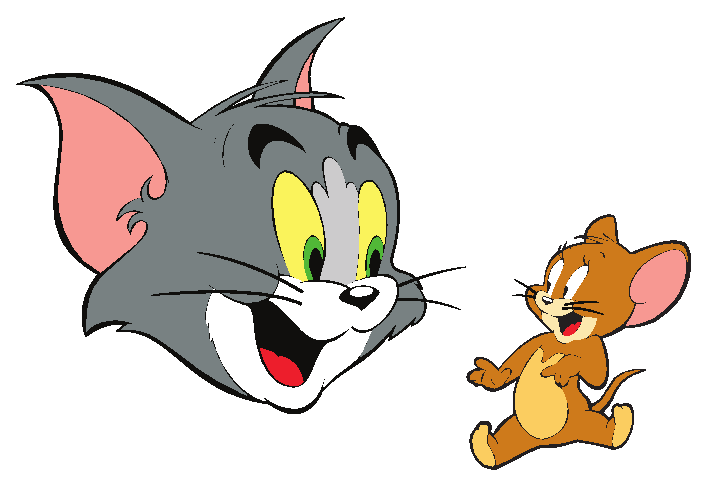
\includegraphics[width=\textwidth]{TomandJerry}
      \caption{Tom and Jerry}
      \label{fig:TomJerry}   
    \end{subfigure}             
    \begin{subfigure}[b]{0.3\textwidth}
      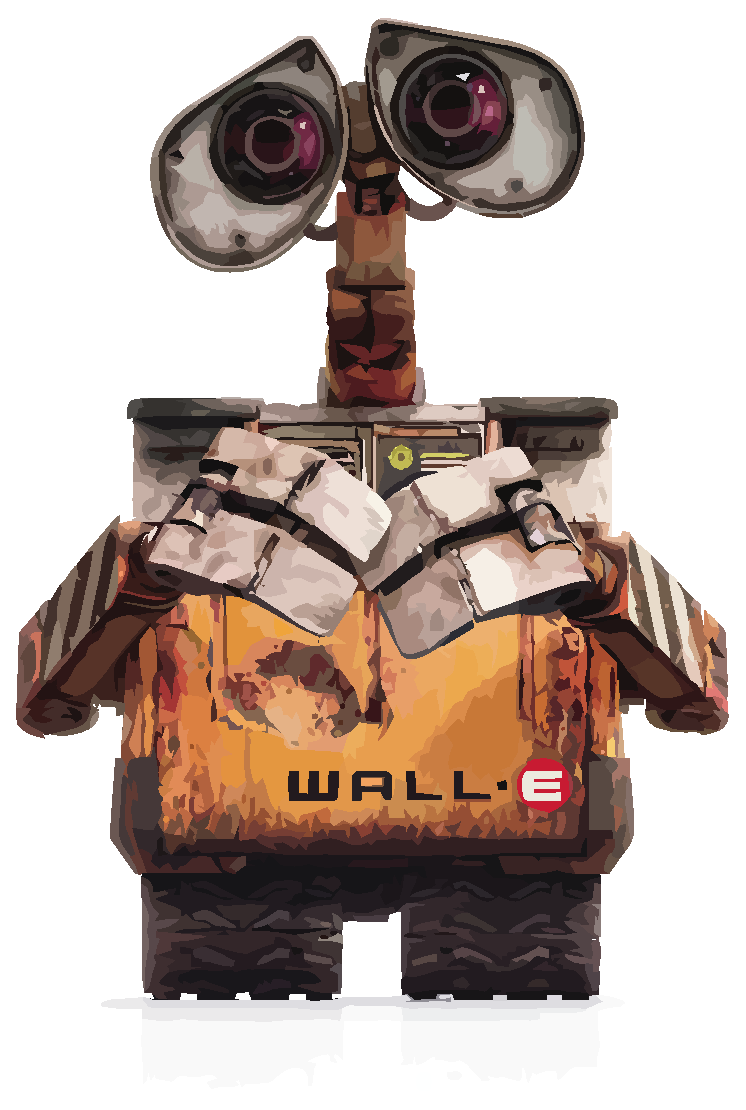
\includegraphics[width=\textwidth]{WallE}
      \caption{Wall-E}
      \label{fig:WallE}
    \end{subfigure}             
    \begin{subfigure}[b]{0.3\textwidth}
      
\includegraphics[width=\textwidth]{minion}
      \caption{Minions}
      \label{fig:Minnion}
    \end{subfigure}
    \caption{Best Animations}
    \label{fig:animations}
  \end{figure}
  
  
  \end{landscape}

\end{comment}
